%%This is a very basic article template.
%%There is just one section and two subsections.
\documentclass{book}
\usepackage[croatian]{babel}
\usepackage[utf8]{inputenc}
\usepackage{amsmath}
\usepackage{graphicx}
\usepackage{pgf}
\usepackage{tikz}
\usepackage{framed, color}
\usetikzlibrary{shapes,arrows,calc,trees,positioning,chains,shapes.geometric,
    decorations.pathreplacing,decorations.pathmorphing,
    matrix,shapes.symbols}

\definecolor{shadecolor}{rgb}{0.83, 0.83, 0.83}

\usepackage{float}

\tikzset{
>=stealth',
  punktchain/.style={
    rectangle, 
    rounded corners, 
    % fill=black!10,
    draw=black, very thick,
    text width=10em, 
    minimum height=3em, 
    text centered, 
    on chain},
  line/.style={draw, thick, <-},
  element/.style={
    tape,
    top color=white,
    bottom color=blue!50!black!60!,
    minimum width=8em,
    draw=blue!40!black!90, very thick,
    text width=10em, 
    minimum height=3.5em, 
    text centered, 
    on chain},
  every join/.style={->, thick,shorten >=1pt},
  decoration={brace},
  tuborg/.style={decorate},
  tubnode/.style={midway, right=2pt},
}


\title{Raspoznavanje uzoraka }
\author{ prof. dr.sc. Slobodan Ribarić }

\begin{document}

\maketitle

\tableofcontents 

\chapter{Uvod}

\marginpar[]{\textbf{Raspoznavanje uzoraka}}
\indent \textbf{ Raspoznavanje uzoraka } (eng. \textit{ Pattern
Recognition}, njem. \textit{ Mustererkennung}, franc. \textit{le reconnaissance des formes})
je znanstvena disciplina Računarskih znanosti  čiji je cilj \textbf{
klasifikacija} ( razvrstavanje) \textbf{objekata} u jedan od brojnih \textbf{
razred} ili \textbf{ klasa}.  \\

\indent Raspoznavanje uzoraka je relativno mlada
znanstvena disciplina nastala 1965. -- 1970. godina. Kao takva, sastavni je dio
umjetne (strojne) inteligencije (eng. \textit{Machine intelligence}). \\


\marginpar[]{\textbf{Primjeri područja \\ upotrebe}} Postoje brojne primjene
\textit{Raspoznavanja uzoraka} u stvarnom životu. Neke zanimljivije primjere možemo pronaći u nekoliko različitih domena. \\

Prilikom raspoznavanja vizualnih objekata možemo izvršavati
\textit{klasifikacija znakova} (slovčano-brojčanih, tiskanih, rukom pisanih,
OCR sustavi), raspoznavati objekte bitne za \textit{medicinsku dijagnostiku}
(X-- mamografija, tomografija, građa stanice, klasifikacija kromosoma),
detektirati i lokalizirati objekte na slikama, interpretirati 3D scene (robotski
ili strojni vid), otkrivati prirodna bogatstava na temelju satelitskih snimaka.
Raspoznavanje uzoraka sastavni je dio \textit{računalnog vida} te
\textit{biometrijskih sigurnosnih sustava}. \\
    
Ako želimo raspoznavati zvučne uzorke, htjet ćemo raspoznavati govor, govornika,
jezika te zvuk (pravilan rad stroja, tip vozila, raspoznavanje koraka). \\
  
Biomedicina predstavlja veliko područje uporabe za raspoznavanje uzoraka.
Pri raspoznavanju biomedicinskih uzoraka raspoznajemo EKG, EEG te
dijagnosticiramo različite bolesti. \\

Raspoznavanjem uzoraka potreba želimo saznati je li potres nastao prirodnim
uzrokom ili je potaknut podzemnom atomskom eksplozijom.Također, želimo
raspoznati korake te razlikovati ljudske od životinjskih. \\
   

Raspoznavanjem ponašanje složenih sustava možemo predviđati vrijeme,
raspoznavati smjerove razvoja te razvoj ponude i potražnje na tržištu. \\


\marginpar[\textbf{Novo znanje}]{\textbf{Novo znanje}} Najnoviji i najznačajniji
 rezultati iz područja \textit{raspoznavanja uzoraka} objavljuju se  u
 međunarodnim znanstvenim časopisima. Evo nekoliko najvažnijih:

\begin{itemize}
  \item IEEE Transactions on Pattern Analysis and Machine Intelligence
  \item IEEE Transactions on Systems, Man and Cybernetics
  \item IEEE Transactions on Neural Networks
  \item IEEE Transactions on Speech and Audio Processing
  \item IEEE Transactions on Image Processing
  \item IEEE Transactions on Fuzzy Systems
  \item Pattern Recognition
  \item Pattern Recognition Letters
  \item Computer Vision and Image Understanding
  \item Computer Speech and Language 
\end{itemize}


\section{Osnovni pojmovi i terminologija}

 
\marginpar{\quad \quad \quad \quad \quad \textbf{Okolina}} \textbf{Okolina}
$\Theta$ je skup predmeta, pojava  i bića, kraće objekata , koje raspoznajemo: 
$$ \Theta = \Theta_B \cup V_{\Theta} $$ gdje  je: $$ \Theta_B = \{ \sigma_k : k
= 1,2, \ldots \}  $$ skup objekata,  a $$ V_{\Theta} = \{ v_j : j = 1,2,\ldots
\} $$ skup međusobnih relacija i  veza između objekata u prostoru i vremenu. \\

Pri tome svaki objekt (predmet, fizička pojava, pojam, činjenica ili
stanje) možemo opisati odgovarajućim brojem funkcija. Vrijednost tih funkcija
daje karakterističnu količinu u prostoru i vremenu (u zavisnosti o vrsti
objekata  i osjetniku ili mjernom uređaju). \\

\marginpar[\quad \quad \quad \quad \quad \textbf{Univerzalni sustav za
raspoznavanje}]{ \textbf{Univerzalni sustav za
raspoznavanje}} \textit{Univerzalni sustav za raspoznavanje} koji je u stanju
procesirati cijelu okolinu ili čak  veći dio okoline \textbf{NIJE IZVEDIV (za
sada)} - zato pri oblikovanju sustava za raspoznavanje uzoraka se ograničavamo
na \textit{područje uporabe}. \\ 
\newpage 

\marginpar[\quad \quad \quad \quad \quad \textbf{Područje uporabe}]{
\textbf{Područje uporabe}} 
\textbf{ Područje uporabe } sadrži
samo one objekte $ \sigma_k \in \Theta_B $ i njihove  međusobne veze i odnose
$v_j \in V_\Theta $ koje raspoznajemo: $$ \mathcal{PU} \in \Theta $$
Skup $\mathcal{PU}$ određen je \textbf{zadatkom} sustava za raspoznavanje. \\

\begin{shaded}
\textit{Primjeri:   \begin{itemize}
  \item raspoznvanje brojeva u rasponu 0 do 9
  \item raspoznavanje slovčanih znakova
  \item raspoznavanje sastavnih djelova određenog složenog proizvoda
  \item raspoznavanje EKG-a
  \item analiza slika dobivenih iz određenog broja spektralnih kanala \\
\end{itemize}}
\end{shaded}

\marginpar[\quad \quad \quad \quad \quad \textbf{Uzorak}]{
\textbf{Uzorak}} \textbf{Uzorak } je generički izraz za objekte  raspoznavanja
(eng. \textit{Pattern}).  Uzorak sadrži rezultat percepcije ili mjerenja (mjerna
naprava, osjetinik) i  predočava stroju podatke o objektu ili objektima i
njihovim međusobnim odnosima $$ f_k(x) = \begin{bmatrix} 
f_{k_1}(x_1, x_2, \ldots, x_q) \\
f_{k_2}(x_1, x_2, \ldots, x_q) \\
\vdots \\
f_{k_p}(x_1, x_2, \ldots , x_q)
\end{bmatrix} $$ 

gdje $p$ i $q$ zavise od sustava osjetnika, odnosno mjernih naprava koje sustav
za raspoznavanje uzoraka koristi. \\

\begin{shaded}
\textit{ Primjeri:  \begin{itemize}
  \item sustav za raspoznavanje EKG signala: \\ f(t); p=q=1, t - vrijeme
  \item sustav za raspoznavanje alfanumeričkih znakova: \\ f(x,y); p=1, q=2
  \item sustav za raspoznavanje objekata u slikama u boji: \\ $f^R(x,y)$,
  $f^G(x,y)$, $f^B(x,y)$; p=3, q=2 \\
\end{itemize} }
\end{shaded}

Funkcija koja preslikava objekt raspoznavanja u uzorak  mora biti takva da
\underline{jednoznačno} objekte iz razreda $\Theta_{B_i}$ preslika u razred
uzoraka $C_i$. \\ 


\textbf{Razred objekata } $ \Theta_{B_i} \subset
\Theta_B; i=1,2,\ldots, M $ \marginpar[  \textbf{Razred objekata}]{
\textbf{Razred objekata}} je podskup onih  objekata iz zadanog područja
uporabe, na koje se odnosi \underline{\textit{oznaka}} (simbol, ime razreda)
$\omega_i$ iz skupa oznaka razreda objekata: $$ \Omega = \{ \omega_1, \omega_2,
\ldots, \omega_M \} .$$ \\

\begin{shaded}
\textit{ Primjer:   Područje uporabe i raspoznavanje voća mogu činiti razredi
označeni oznakam ``banana'', `` limun'', ``kruška``, \ldots, itd. } \\
\end{shaded}


Za zadano područje uporabe broj razreda $M \geq 2 $ je određen zadatkom sustava
za raspoznavanje (možemo reći da je $M$ apriorno poznat), te 
vrijedi: $$ \Theta_{B_i} \cap \Theta_{B_j} = \emptyset \ za \ \forall i \neq j
$$ $$ \bigcup\limits^{M}_{i=1} \Theta_{B_i} = \Theta_B $$ \\

Presjek više razreda objekata mora biti prazan skup. Drugim rječima, jedan
objekt može istovremeno pripadati \textbf{samo jednom} razredu objekata.
Također, a djelomično slijedi iz gornjeg, unija svih razreda objekata mora
činiti potpun skup objekata $\Theta_B$. \\

\marginpar[  \textbf{Razred uzoraka}]{ \textbf{Razred uzoraka}} \textbf{Razred
uzoraka} $C_i$ čine slike objekata iz razreda  $\Theta_{B_i}; i =1,2,\ldots,M$.
Za zadano područje uporabe $\mathcal{PU}$ mora vrijediti za  svaki par razreda
uzoraka $(C_i, C_j)$ da je $$ C_i \cap C_j = \emptyset \ za \ \forall i \neq j $$
te da je svaki uzorak iz razreda $C_i$  sličniji nekom  drugom uzorku iz razreda
$C_i$, negoli uzorku iz razreda $C_j$ za $\forall i \neq j $. \\

 \marginpar[  \textbf{Opisivanje područja uporabe}]{ \textbf{Opisivanje
 područja uporabe}} \textbf{ Skup uzoraka koji opisuje područje uporabe } čini
 konačan broj uzoraka iz zadanog područja  uporabe. Taj konačan  skup $S_N$ koji
 čine $M$ podskupova uzoraka $S_i$ mora zadovoljavati slijedeće uvjete:
\begin{itemize}
  \item $S_i \subseteq C_i, \ za \ \forall i=1,2,\ldots, M $
  \item $S_i \neq \emptyset, \ za \ \forall i=1,2,\ldots, M$
  \item $S_i \cap S_j = \emptyset, \ za \ \forall i \neq j$
  \item $\bigcup\limits^{M}_{i=1}S_i = S_N $
\end{itemize}
gdje je $C_i$ $i$-ti razred uzoraka iz zadanog područja uporabe. S $N_i$
označimo kardinalni broj podskupa $S_i$. Za $N$ - kardinalni broj skupa $S_N$,
 vrijedi:
$$ N = \sum\limits^{M}_{i=1}N_i .$$ \\

\marginpar[\textbf{ Skup za  učenje}]{
 \textbf{Skup za učenje}} 
 \textbf{Skup uzoraka za učenje }  $U_M$   je konačan skup uzoraka iz zadanog
 područja uporabe $\mathcal{PU}$, iz kojeg sustav  za raspoznavanje  uzoraka
 može \textit{naučiti} veze  između  oznake  razreda i objekata  raspoznavanja: $$
 U_M = ( S_N, \Omega) $$  gdje  je $S_N$ skup uzoraka koji  opisuje područje 
 uporabe,  a $\Omega = \{ \omega_1, \omega_2, \ldots, \omega_M \}$ skup   oznaka
 razreda objekata u zadanom području uporabe. \\

Skup za učenje sastoji se od $podskupova$ koje sačinjavaju parovi $(uzorak,
klasa)$, a unutar jednog podskupa $U_i$ svi uzorci pripadaju klasi $\omega_i$:

$$U_M = \{ U_1, U_2, \ldots, U_M \}$$ 
gdje je 
$$ U_i = \{ ( f_{i_1}( \vec{x} ), \omega_i ), ( f_{i_2}( \vec{x} ), \omega_i) ,
\ldots, ( f_{i_N}( \vec{x} ), \omega_i ) \}. $$ 

\noindent Pri tome moraju biti ispunjeni slijedeći uvjeti: 
\begin{itemize}
  \item $U_i \neq \emptyset \ za \ \forall i=1,2,\ldots, M $
  \item uzorci iz $U_i$ moraju biti međusobno slični
  \item uzorci iz $U_i$ nisu slični uzorcima iz $U_j$ za $ \forall
  i=1,2,\ldots, M$
  \item $U_i \cap U_j = \emptyset \ za \ \forall i \neq j$
  \item $\bigcup\limits^{M}_{i=1} U_i = U_M$ \\
\end{itemize}

Uzorke iz $S_N$ u procesu oblikovanja sustava za raspoznavanje
uzoraka za zadano područje uporabe, izabire i označava čovjek - stručnjak za
zadano područje uporabe ( nazovimo ga \textit{učitelj}). \\

\marginpar[  \textbf{Učenje}]{ \textbf{Učenje}} \textbf{Učenje
} je proces u kojem se upostavljaju veze između uzoraka iz skupa za učenje i
oznakama razreda uzoraka.  Učenje izvodimo s nepotpunom indukcijom pomoću koje
poopćujemo informaciju (koju sadrži relativno  mali skup za učenje) na sve uzorke iz danog
područja uporabe $\mathcal{PU}$.  \\
\newpage

\begin{shaded}
\textit{Primjer:  } \\

\begin{figure}[H]
\begin{center}

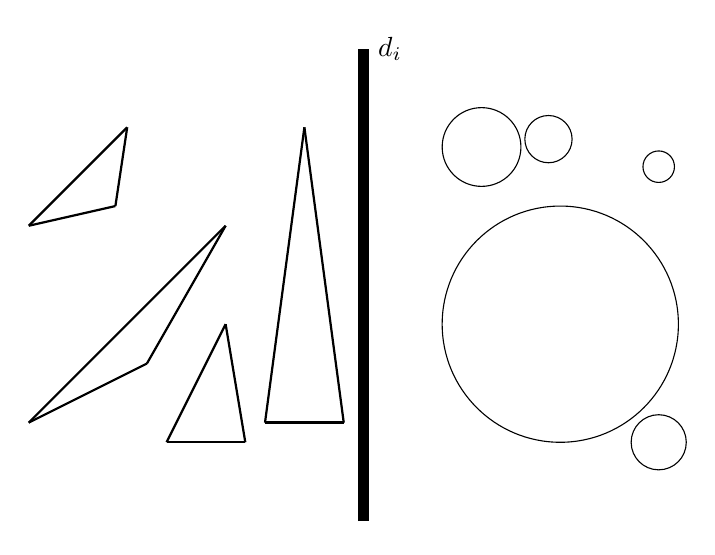
\begin{tikzpicture}[
    scale=5,
    axis/.style={very thick, ->, >=stealth'},
    important line/.style={thick},
    dashed line/.style={dashed, thin},
    pile/.style={thick, ->, >=stealth', shorten <=2pt, shorten
    >=2pt},
    every node/.style={color=black}
    ]
    
   
    % Triangles
    \draw[important line] (.15,.15)  -- (.65,.65)
         node[right, text width=5em] {};
    \draw[important line] (.65,.65)  -- (.45,.30)
         node[right, text width=5em] {};
    \draw[important line] (.15,.15)  -- (.45,.30)
         node[right, text width=5em] {};
         
         
    \draw[important line] (.15,.65)  -- (.4,.9)
         node[right, text width=5em] {};
    \draw[important line] (.37,.7)  -- (.4,.9)
         node[right, text width=5em] {};
    \draw[important line] (.15,.65)  -- (.37,.7)
         node[right, text width=5em] {};
         
         
    \draw[important line] (.75,.15)  -- (.85,.9)
         node[right, text width=5em] {};
    \draw[important line] (.85,.9)  -- (.95,.15)
         node[right, text width=5em] {};
    \draw[important line] (.95,.15)  -- (.75,.15)
         node[right, text width=5em] {};
         
         
    \draw[important line] (.5,.1)  -- (.7,.1)
         node[right, text width=5em] {};
    \draw[important line] (.7,.1)  -- (.65,.4)
         node[right, text width=5em] {};
    \draw[important line] (.65,.4)  -- (.5,.1)
         node[right, text width=5em] {}; 
    
    %circles
    
    \draw (1.5, 0.4) circle (.3); 
    
    \draw (1.3, 0.85) circle (.1); 
    
    \draw (1.75, 0.1) circle (.07);  
    
    \draw (1.75, 0.8) circle (.04);  
    
     \draw (1.47, 0.87) circle (.06);     
         
    %decision function    
    \draw[line width=4pt] (1,-0.1)  -- (1,1.1)
         node[right, text width=5em] {$d_i$};
   
    
\end{tikzpicture}


 razred ``trokut'' \quad \quad \quad \quad \quad \quad      razred ``krug''
\end{center}
\end{figure}

\begin{figure}[H]
\begin{center}

\begin{tikzpicture}[
    scale=5,
    axis/.style={very thick, ->, >=stealth'},
    important line/.style={thick},
    dashed line/.style={dashed, thin},
    pile/.style={thick, ->, >=stealth', shorten <=2pt, shorten
    >=2pt},
    every node/.style={color=black}
    ]
    
    \draw[important line] (.15,.15)  -- (.4,.64)
         node[right, text width=5em] {};
    \draw[important line] (.4,.65)  -- (.45,.30)
         node[right, text width=5em] {};
    \draw[important line] (.15,.15)  -- (.45,.30)
         node[right, text width=5em] {};
         
     \draw (.8, 0.4) circle (.1); 
     
    \draw (1.4, 0.6) circle (.17); 
    
    \draw[important line] (1.63,.3)  -- (1.84,.76)
         node[right, text width=5em] {};
    \draw[important line] (1.84,.76)  -- (1.9,.15)
         node[right, text width=5em] {};
    \draw[important line] (1.9,.15)  -- (1.63,.30)
         node[right, text width=5em] {};
    
    
\end{tikzpicture}

 Ispitni primjeri geometrijskih likova 
\end{center}

\end{figure}

\end{shaded}



\marginpar[  \textbf{Tipovi uzoraka}]{ \textbf{Tipovi uzoraka}} 
Uzorke možemo podijeliti u dvije velike skupine bazirane na kompleksnosti
informacije koju sadrži. To su \textit{jednostavni} i \textit{složeni} uzorci.
\\

Uzorak je \textbf{jednostavan} ako ga raspoznajemo  kao cjelinu (korisnik
sustava za raspoznavanje uzoraka je zainteresiran samo za oznaku razreda kojem
uzorak pripada). Uzorak se smatra \textbf{složenim} ako samo ime razreda nije
dovoljno korisniku sustava za raspoznavanje uzoraka ili je čak klasifikacija
uzorka neizvediva. \\

\begin{shaded}
\textit{Primjer:  \begin{itemize}
  \item slika jednog slova ili znaka $\rightarrow$ jednostavan uzorak
  \item slika jedne stranice teksta $\rightarrow$ složeni uzorak
  \item signal izgovorene riječi $\rightarrow$ jednostavan uzorak
  \item signal izgovorene priče $\rightarrow$ složeni uzorak \\
\end{itemize}}
\end{shaded}


\marginpar[  \textbf{Raspoznavanje jednostavnih uzoraka}]{
\textbf{Raspoznavanje jednostavnih uzoraka}} Raspoznavanje
jednostavnih uzoraka možemo definirati kao
 $$RU \ : \ f_k( \vec{x} ) \longmapsto \omega_l, \ \omega_l \in \Omega $$  
gdje  je $\Omega$ skup od $M$ uzoraka razreda iz $PU$.  \textit{ Vrlo često se
prirodaje $M+1$ oznaka oznaka koja označava razreda  odbačenih uzoraka koje
sustav ne može raspoznati.} \\

\marginpar[  \textbf{Raspoznavanje složenih uzoraka}]{
\textbf{Raspoznavanje složenih uzoraka}} Raspoznavanje
složenih uzoraka definiramo kao 
$$ RU \ : \ f_k( \vec{x} ) \longmapsto \lambda_l, $$ 
gdje je $\lambda_l$ koristan  opis uzorka (eng. \textit{pattern description,
pattern interpretation}). Kao rezultat raspoznavanja složenih uzoraka možemo
dobiti \textit{popis predmeta ili događaja koji su predmet zanimanja}, \textit{
opis promjena utvrđenih iz vremenskih sljedova uzoraka} te  \textit{opis
sastavaljen iz definicije znakova ili riječi nekog prirodnog ili umjetnog
jezika}. \\



\section{Šest postulata raspoznavanja uzoraka}

\marginpar[  \textbf{Šest postulata}]{
\textbf{Šest postulata}} Pri prikupljanju uzoraka za naš sustav moramo obratiti pažnju na nekoliko
pravila. Ta pravila možemo formulirati u \textit{šest postulata raspoznavanja
uzoraka: } \\
\begin{itemize}
  \item \underline{\textbf{Postulat 1: }} U cilju prikupljanja informaciju o
  $PU$ moraju biti raspoloživi reprezentativni uzorci iz $M$ razreda
  \item \underline{\textbf{Postulat 2: }} Jednostavan uzorak ima značajke koje
  karakteriziraju njegovu pripadnost razredu
  \item \underline{\textbf{Postulat 3: }} Značajke uzoraka koji pripadaju
  jednom razredu uzoraka zauzimaju kompaktno područje u prostoru značajki.
  Područja okupirana značajkama različitih razreda su odvojena
  \item \underline{\textbf{Postulat 4: }} Složeni uzorak sastoji se iz
  jednostavnijih građevnih komponenti ili segmenata objekata koji se nalaze u
  izvjesnim odnosima. Uzorak se može sastaviti od tih komponenti
  \item \underline{\textbf{Postulat 5: }} Složeni uzorak koji pripada određenom
  području uporabe ima određenu strukturu. To implicira da bilo kakvo uređenje
  jednostavnih građevnih elemenata neće dati uzorak $f_k(\vec{x})$
  \item \underline{\textbf{Postulat 6: }} Dva uzorka su si slična ako je pogodno
  definirana mjera udaljenosti u prostoru značajki mala
\end{itemize}







\chapter{Model sustava za raspoznavanje uzoraka}

\section{Formalni model}

\begin{figure}[H]
\begin{center}

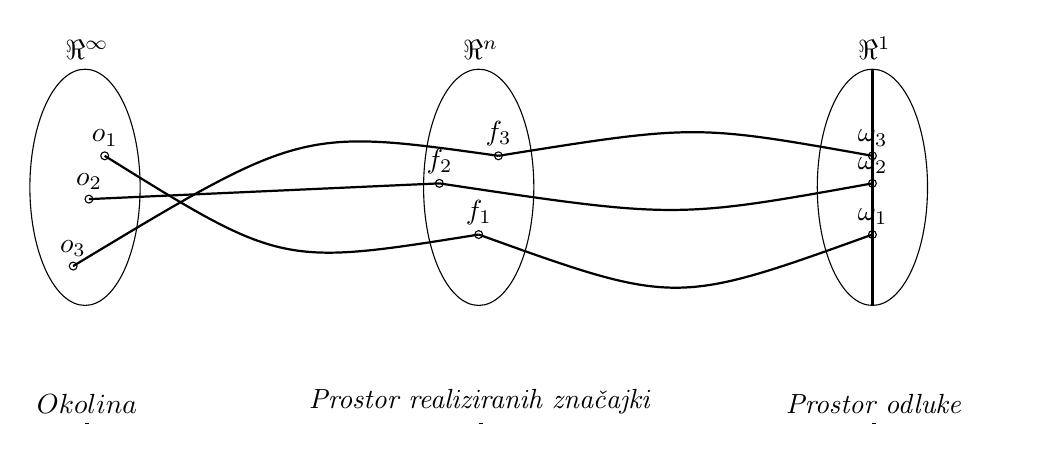
\begin{tikzpicture}[
    scale=5,
    axis/.style={very thick, ->, >=stealth'},
    important line/.style={thick},
    dashed line/.style={dashed, thin},
    pile/.style={thick, ->, >=stealth', shorten <=2pt, shorten
    >=2pt},
    every node/.style={color=black}
    ]
    
    %first domain
    \draw (0, 0) ellipse (.14 and .3);
    \draw (0,0.3) -- (0.01,0.3) node[pos=.5,sloped,above] {$\Re^\infty$};
    \draw (0,-0.6) -- (0.01,-0.6) node[pos=.5,sloped,above] {$Okolina$};
     
    \draw (.05, .08) circle (.01);
    \draw (.05,0.08) -- (0.051,0.08) node[pos=.5,sloped,above] {$o_1$};
    
    \draw (.01, -.03) circle (.01);
    \draw (.01,-.03) -- (0.011,-.03) node[pos=.5,sloped,above] {$o_2$};
    
    \draw (-.03, -.2) circle (.01);
    \draw (-.03,-.2) -- (-.031,-.2) node[pos=.5,sloped,above] {$o_3$};
    
    %second domain
    \draw (1, 0) ellipse (.14 and .3);
    \draw (1,0.3) -- (1.01,0.3) node[pos=.5,sloped,above] {$\Re^n$};
    \draw (1,-0.6) -- (1.01,-0.6) node[pos=.5,sloped,above] {\textit{Prostor 
    realiziranih  značajki}};
    
    \draw (1.05, .08) circle (.01);
    \draw (1.05,0.08) -- (1.051,0.08) node[pos=.5,sloped,above] {$f_3$};
    
    \draw (0.9, .01) circle (.01);
    \draw (0.9,0.01) -- (.901,0.01) node[pos=.5,sloped,above] {$f_2$};
    
    \draw (1, -.12) circle (.01);
    \draw (1,-.12) -- (1.001,-.12) node[pos=.5,sloped,above] {$f_1$};
    
    
    %third domain
    \draw (2, 0) ellipse (.14 and .3);
    \draw (2,0.3) -- (2.01,0.3) node[pos=.5,sloped,above] {$\Re^1$};
    \draw[line width=1pt] (2,-0.3)  -- (2,0.3) 
         node[right, text width=5em] {};
   \draw (2,-0.6) -- (2.01,-0.6) node[pos=.5,sloped,above] {\textit{Prostor 
   odluke}};
    
    \draw (2, -.12) circle (.01);
    \draw (2,-.12) -- (2.001,-.12) node[pos=.5,sloped,above] {$\omega_1$};
    
    \draw (2, .01) circle (.01);
    \draw (2,0.01) -- (2.001,0.01) node[pos=.5,sloped,above] {$\omega_2$};
    
    \draw (2, .08) circle (.01);
    \draw (2,0.08) -- (2.001,0.08) node[pos=.5,sloped,above] {$\omega_3$};



	%connections
	
	\draw[important line] (.05, .08) .. controls (.5, -.2) .. (1, -.12) ;
	\draw[important line] (.01, -.03) to (0.9, .01) ;
	\draw[important line] (-.03, -.2) .. controls (.55, .15) .. (1.05, .08) ;
	
	\draw[important line] (1, -.12) .. controls (1.5, -.3) .. (2, -.12) ;
	\draw[important line] (0.9, .01) .. controls (1.5, -.08) .. (2, .01) ;
	\draw[important line] (1.05, .08) .. controls (1.55, .16) .. (2, .08) ;
	
	\draw[line width=1pt] (2,-0.3)  -- (2,0.3)
         node[right, text width=5em] {};
	
\end{tikzpicture}

\caption{ Formalni model sustava za raspoznavanje uzoraka}
\end{center}
\end{figure}





U formalnom modelu sustava za raspoznavanje uzoraka, u okolini $\Theta$
pronalazimo objekte i veze među njima:  $\sigma_k \in \Theta$, $v_j \in
V_{\Theta}$. Postupkom \marginpar[\textbf{Mjerenje}]{\textbf{Mjerenje}}
\textit{mjerenja} iz okoline uzorkujemo objekte i  pretvaramo ih u značajke
$f_k$ : $\sigma_k \rightarrow f_k$. Time dobivamo  \textbf{ prostor realiziranih
uzoraka.} 
Postupkom \marginpar[\textbf{Klasifikacija}]{\textbf{Klasifikacija}}
\textit{klasifikacije} dobivene   uzorke smještamo u jednu od  mogućih klasa, 
te  dobivamo \textbf{prostor razreda  uzoraka: }  $\Omega = \{ \omega_1, \ldots,
\omega_M \}$. \\

Postupak redukcije značajki možemo zorno prikazati \textit{Uhrovim stožcem
raspoznavanja} prikazanim na slici 2.2. 

\begin{figure}[H]
\begin{center}

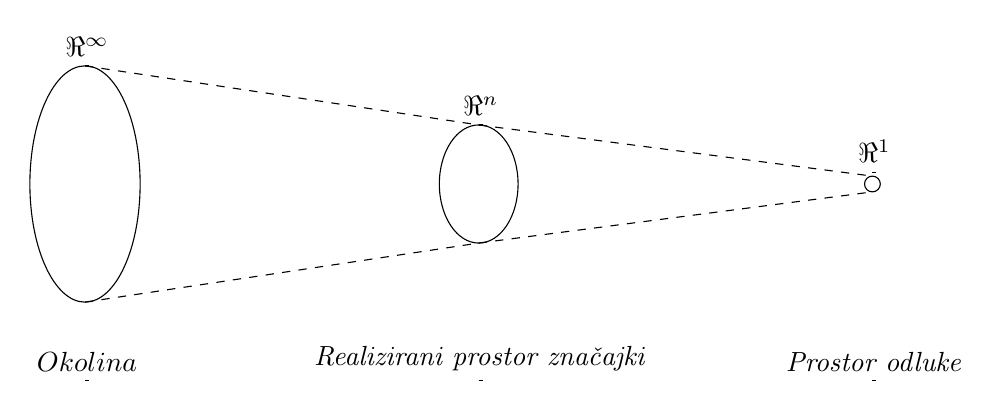
\begin{tikzpicture}[
    scale=5,
    axis/.style={very thick, ->, >=stealth'},
    important line/.style={thick},
    dashed line/.style={dashed, thin},
    pile/.style={thick, ->, >=stealth', shorten <=2pt, shorten
    >=2pt},
    every node/.style={color=black}
    ]

	\draw (0, 0) ellipse (.14 and .3);
	\draw (0,0.3) -- (0.01,0.3) node[pos=.5,sloped,above] {$\Re^\infty$};
	\draw (0,-0.5) -- (0.01,-0.5) node[pos=.5,sloped,above] {$Okolina$};
	
	\draw (1, 0) ellipse (.1 and .15);
	\draw (1,0.15) -- (1.01,0.15) node[pos=.5,sloped,above] {$\Re^n$};
	\draw (1,-0.5) -- (1.01,-0.5) node[pos=.5,sloped,above] {\textit{Realizirani
	 prostor  značajki}};
	
	\draw (2, 0) circle (0.02);
	\draw (2,0.03) -- (2.01,0.03) node[pos=.5,sloped,above] {$\Re^1$};
	\draw (2,-0.5) -- (2.01,-0.5) node[pos=.5,sloped,above] {\textit{Prostor
	odluke}};
	
	\draw[dashed] (0,0.3) -- (1,0.15);
	\draw[dashed] (0,-0.3) -- (1,-0.15);
	
	\draw[dashed] (1,0.15) -- (2,0.02);
	\draw[dashed] (1,-0.15) -- (2,-0.02);

\end{tikzpicture}

\caption{Uhrov stožac raspoznavanja -- redukcija značajki}
\end{center}
\end{figure}




\section{Značajke, vektor značajki i klasifikator}


\tikzstyle{block} = [draw, fill=blue!20, rectangle, 
    minimum height=3em, minimum width=6em]
\tikzstyle{sum} = [draw, fill=blue!20, circle, node distance=1cm]
\tikzstyle{input} = [coordinate]
\tikzstyle{output} = [coordinate]
\tikzstyle{pinstyle} = [pin edge={to-,thin,black}]


\begin{figure}[H]
\begin{center}

\begin{tikzpicture}[auto, node distance=2cm,>=latex']
    % We start by placing the blocks
    \node [input, name=input] {};
    
    \node [block, right of=input] (senzor) {Senzor};
    \node [block, right of=senzor, pin={[pinstyle] below:},
            node distance=3cm] (generiranje) {Generiranje };
    \node [block, right of=generiranje, pin={[pinstyle] below:},
            node distance=3cm] (izbor) {Izbor};
    \node [block, right of=izbor, pin={[pinstyle] below:},
            node distance=3cm] (oblikovanje) {Oblikovanje};
    \node [block, right of=oblikovanje,
            node distance=3cm] (evaluacija) {Evaluacija};
            
            
    \draw [draw,<->] (evaluacija) -- +(0, -1) -| (senzor);    
    \draw [draw,->] (senzor) --  (generiranje);
    \draw [draw,->] (generiranje) --  (izbor);
    \draw [draw,->] (izbor) --  (oblikovanje); 
    \draw [draw,->] (oblikovanje) --  (evaluacija);
    

    
\end{tikzpicture}

\caption{Osnove faze u postupku oblikovanja sustava RU}
\end{center}
\end{figure}








Informacije o objektima iz fizičkog svijeta formiramo u
\marginpar[\textbf{Značajke}]{\textbf{Značajke}} \textbf{značajke}.
Značajke promatramo kao slučajne varijable $x_i$. \\ 

Značajke jednog objekta formiramo u
\marginpar[\textbf{Vektor značajki}]{\textbf{Vektor značajki}} \textbf{vektor
značajki}. Vektor značajki promatramo kao slučajni vektor $\vec{x}$: 
$$ \vec{x} =  [ x_1, x_2, \ldots, x_n ]^T $$

\marginpar[\textbf{Tipovi značajki}]{\textbf{Tipovi značajki}} Značajke možemo
podijeliti u dvije skupine - \textit{interset} i \textit{intraset}. \\


Značajke koje predstavljaju razlike između razreda uzoraka nazivaju se
\textbf{interset} značajkama i to su značajke koje nose informacije potrebne za
klasifikaciju objekata. \\

\textbf{Intraset} značajke zajedničke su  \textbf{svim} razredima iz
$\mathcal{PU}$ (područja uporabe) i \underline{ne nose}  diskriminacijsku
informaciju -- \textbf{takve značajke mogu se zanemariti}. \\

\newpage

\marginpar[\textbf{Izbor značajki}]{\textbf{Izbor značajki}} Kada biramo
značajke koje će čini \textit{skup za učenje}, biramo \textit{interset}
značajke. Pri tome ne smijemo zaboraviti da je u većini slučajeva  određivanje
potpunog skupa diskriminacijskih značajki \textbf{iznimno teško ili čak
nemoguće}. Neke diskriminacijske značajke mogu se naći na temelju raspoloživih 
rezultata mjerenja (senzoriranja). \\

Vektor značajki predočujemo kao točku u $n$--dimenzijskom prostoru značajki.
Obično definiramo i neku vrstu metrike u takvom prostoru značajki. Često ćemo se
susresti s velikim brojem značajki te ćemo htjeti smanjiti dimenzionalnost
prostora značajki. Redukciju dimenzionalnosti vektora značajki postižemo
uporabom različitih transformacija uz minimalni gubitak informacija. \\


Klasifikaciju samog uzorka temeljimo na decizijskim funkcijama, te se susrećemo
s problemom određivanja optimalne decizijske procedure. Problem  klasifikacije
može se promatrati kao razvrstavanje  nepoznatog uzorka u potprostor prostora
značajki na temelju decizijskih granica koje definiraju te procedure. \\


\marginpar[\textbf{Pravilo razvrstavanja}]{\textbf{Pravilo
razvrstavanja}} Decizijske granice određene su decizijskim funkcijama:
$d_1(\vec{x}), d_2(\vec{x}), \ldots, d_n(\vec{x})$. Važno  je zapamtiti da je
\textit{$d_i$ funkcija koja ima za argument \textbf{vektor}  a vraća
\textbf{skalar}}. Sada možemo definirati i \textbf{pravilo razvrstavanja: } 
\begin{shaded}

\textit{ Ako $d_i(\vec{x}) > d_j(\vec{x})$ za $i,j = 1,2, \ldots,M$ te $i \neq
j$ tada nepoznati uzorak $\vec{x}$ pripada razredu $\omega_i$}
\end{shaded}


 \begin{figure}[H]
 \begin{center}
 \includegraphics[scale=0.5]{blok}
 \caption{Blok dijagram klasifikatora}
 \end{center}
 \end{figure}

Vratimo se još jednom osnovnim fazama u postupku sustava za raspoznavanje
uzoraka.

\begin{figure}[H]
 \begin{center}
 \includegraphics[scale=0.5]{./pics/faze_second}
 \caption{Osnove faze u postupku oblikovanja sustava RU}
 \end{center}
 \end{figure}

Primjetimo slijedeće stvari. Vanjski fizički svijet je tzv. \textit{analogni
svijet}, i sadrži praktički $\infty$ mnogo značajki ($\Re^{\infty}$). Senzor ili
pretvarač pretvara analogni svijet u zapis koji sadrži $r$ vrijednosti ($\Re^{r}$).
Postupkom \textit{pretprocesiranja} izlučujemo šum i poboljšavamo mjerna
svojstva podataka. \textit{Izlučivanjem značajki} taj prostor dodatno smanjujemo
na prostor s $n$ vrijednosti ($\Re^{r}$, $n << r$), te dobivamo konačni vektor
značajki $\vec{x} = [ x_1, x_2, \ldots, x_n ]^T$. Donošenjem
odluke \textit{pravilom odlučivanja} dolazimo u \textbf{prostor odlučivanja} sa
samo jednom dimenzijom ($\Re^{1}$) - \textit{odlukom}.

\section{Case study: automatska dijagnoza EKG signala na testu opterećenja} 

Pogledajmo slijedeći primjer iz biomedicinske domene. Promatrat ćemo signal
EKG-a pacijenata na testu opterećenja, tj. provodit ćemo automatizaciju
\textit{Lesterove dijagnostičke metode}.  Definirajmo prvo osnovne pojmove.
\\

Područje uporabe $\mathcal{PU}$ je \textit{automatska dijagnoza signala EKG-a u
testu opterećenja}. \\ 

Objekti iz skupa objekata $\Theta_B = \{ \sigma_k; k=1,2, \ldots, n \}$ su
$\sigma_i$ = \textit{signal EKG-a pacijenata}. \\

Koristit ćemo jednostavan uzorak koji će se sastojati od dvije značajke: 
$$ f_k(\vec{x}) \longmapsto \vec{x} = \begin{bmatrix}
x_1 \\
x_2
\end{bmatrix} $$ \\

Moramo još definirati razred objekata, skup oznaka te razred uzoraka. Razred
objekata sastoji nam se od tri oznake:
\begin{itemize}
  \item Normalni EKG
  \item Granični EKG 
  \item Nenormalni EKG
\end{itemize}

Skup oznaka sastoji se od oznaka istoimenih objekata iz razred objekata. Razred
uzoraka sastoji se od slijedećih klasa:
\begin{itemize}
  \item \textbf{ $C_1$ / $\omega_1$} - normalni EKG
  \item \textbf{ $C_2$ / $\omega_2$} - granični EKG
  \item \textbf{ $C_3$ / $\omega_3$} - nenormalni EKG \\
\end{itemize}

EKG signal iz fizičkog svijeta prikazan je na slici 2.6., a izmjereni
(uzorkovani) signal dobiven A/D konverzijom prikazan je na slici 2.7. 

\begin{figure}[H]
 \begin{center}
 \includegraphics[scale=0.5]{./pics/EKGsignal}
 \caption{Signal iz fizičkog svijeta}
 \end{center}
 \end{figure}

\begin{figure}[H]
 \begin{center}
 \includegraphics[scale=0.5]{./pics/EKGsignal_uzorkovan}
 \caption{Uzorkovani signal ($f_u = 800 Hz$)}
 \end{center}
 \end{figure}
 
U procesu pretprocesiranja prije svega želimo eliminirati
\textit{ekstrasistolu} jer to predstavlje smetnju u radu srca koja nam ne donosi
puno informacije, te utvrditi broj otkucaja srca u minuti. Zatim, želimo
detektirati stavilne točke, tj. minimalnu i maksimalnu derivaciju, te filtrirati
usrednjavanjem pri čemu eliminiramo šum za faktor $\sqrt{n}$, gdje je $n$ broj
analiziranih perioda.  \\

Značajke izlučujemo u skladu s Lesterovom dijagnostičkom metodom, te su nam
značajke \textbf{koljeno \textit{J}} i \textbf{spojnica \textit{ST}}. Značajku
$x_1$ nam predtavlja nagib segmenta $ST$, a značajka $x_2$ je depresija koljena
$J$.

\begin{figure}[H]
 \begin{center}
 \includegraphics[scale=0.5]{./pics/znacajke}
 \caption{Prikaz značajki}
 \end{center}
 \end{figure}
 
Prilikom ekstrakcije značajki susrećemo se s dva problema. Prvi problem je što
koljeno $J$ ima različite oblike. Drugi problem je što se segment $ST$ nalazi
između kraja vala $S$ i početka vala $T$ te duljina segmenta $ST$ ovisi o
frekvenciji signala EKG-a, tj. broju otkucaja u minuti.

\begin{figure}
 \begin{center}
 \includegraphics[scale=0.5]{./pics/primjerJiST}
 \caption{Primjeri kliničkih oblika koljena $J$ i nagiba segmenata $ST$}
 \end{center}
 \end{figure}

Tako dobiven prostor značajki prikazan je na slici 2.10., a primjer decizijskih
funkcija za zadani prostor značajki prikazan je na slici 2.11.

\begin{figure}[H]
 \begin{center}
 \includegraphics[scale=0.5]{./pics/prostorZnacajki}
 \caption{Prostor značajki}
 \end{center}
 \end{figure}

\begin{figure}[H]
 \begin{center}
 \includegraphics[scale=0.5]{./pics/decizijskeFunkcije}
 \caption{Prostor značajki razdvojen decizijskim funkcijama}
 \end{center}
 \end{figure}
 
\chapter{Linearne funkcije odlučivanja}

\marginpar[\textbf{Funkcije odlučivanja}]{\textbf{Funkcije odlučivanja}}
Prisjetimo se, osnovni zadatak sustava za raspoznavanje  uzoraka je
razvrstavanja uzoraka u razrede uzoraka.  To izvršavamo pomoću funkcija  koje
dijele prostor uzoraka u područja tako da svako područje pripada samo jednom
razredu uzoraka.  Takve funkcije zovemo \textbf{funkcije odlučivanja} (eng.
\textit{decision functions, discriminant functions}). \\

Ako imamo $N$ razreda uzoraka, moramo imati i jednako toliko funkcija
odlučivanja $d_k(\vec{x}), \ k=1,2,\ldots,N$, tako da vrijedi:
$$ d_i(\vec{x}) > d_j(\vec{x}), \ \forall\vec{x} \in \omega_i, \ i \neq j $$

To nam govori da funkcija odlučivanja $d_i(\vec{x})$ ima najveću vrijednost na
području kojem pripadaju uzorci iz razreda $\omega_i$. Za točke koje se nalaze
na granici prostora $\omega_i$ i $\omega_j$ vrijedi $d_i(\vec{x}) =
d_j(\vec{x})$. Prema tome zaključujemo da će nam za razdvajanje $N$ razreda
trebati $\frac{N(N-1)}{2}$ granica. Treba primjetiti da izbor funkcije
odlučivanja nije jedinstven te da se funkcije odlučivanja mogu zapisati u
različitim oblicima.

\section{Linearne funkcije odlučivanja}

\marginpar[\textbf{Linearna \\ funkcija odlučivanja}]{\textbf{Linearna \\
funkcija odlučivanja}}Najjednostavniji oblik funkcije odlučivanja predstavlja \textbf{linearna funkcija}:
$$ d(\vec{x}) = w_1x_1 + w_2x_2 + \ldots + w_nx_n + w_{n+1}
= \vec{\mathbf{w}}^T\vec{\mathbf{x}} + w_{n+1} $$

\marginpar[\textbf{Koeficijent praga}]{\textbf{Koeficijent praga}} gdje je
$\vec{\mathbf{w}}$ \textbf{vektor težinskih koeficijenata},   $\vec{x}$
\textbf{uzorak} a $w_{n+1}$ \textbf{koeficijent praga}   ili
\textbf{pomak} (eng. \textit{bias, threshold weight}). \\

\marginpar[\textbf{Dimenzionalnost \\ funkcije}]{\textbf{Dimenzionalnost \\
funkcije}}Dimenzionalnost funkcije odlučivanja ovisi o broju razreda kojim
raspolažemo. Za $n=2$ funkcija odlučivanja  je \textit{pravac}, za $n=3$
\textit{ravnina}, a za $n > 3$ funkcija odlučivanja je \textit{hiperravnina}. \\

\begin{figure}[H]
\begin{center}


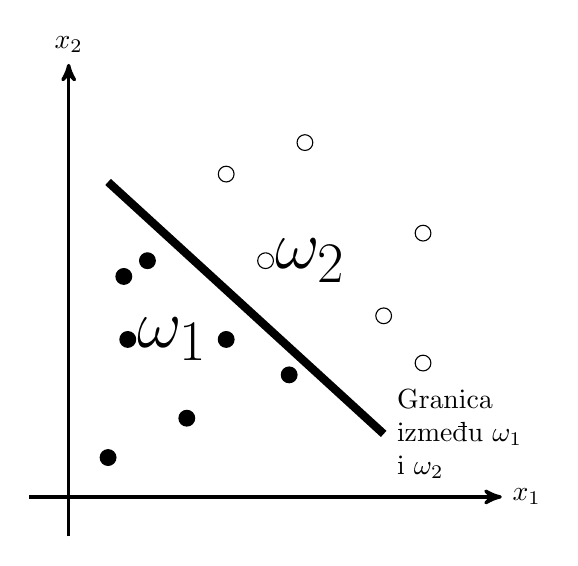
\begin{tikzpicture}[
    scale=5,
    axis/.style={very thick, ->, >=stealth'},
    important line/.style={thick},
    dashed line/.style={dashed, thin},
    pile/.style={thick, ->, >=stealth', shorten <=2pt, shorten
    >=2pt},
    every node/.style={color=black}
    ]

	%axis
	\draw[axis] (-0.1,0)  -- (1.1,0) node(xline)[right]
        {$x_1$};
    \draw[axis] (0,-0.1) -- (0,1.1) node(yline)[above] {$x_2$};
        
    %decision function
    \draw[line width=3pt] (0.1, 0.8) -- (0.8, 0.16)  node[right, text width=5em]
    {Granica između $\omega_1$ i $\omega_2$};
    
    %dots
    
    \draw[fill=black] (0.1, 0.1) circle (0.02);
    \draw[fill=black] (0.15, 0.4) circle (0.02) node[right, text width=5em]
    { \Huge $\omega_1$};
    \draw[fill=black] (0.4, 0.4) circle (0.02); 
    \draw[fill=black] (0.2, 0.6) circle (0.02) ;
    \draw[fill=black] (0.3, 0.2) circle (0.02);
    \draw[fill=black] (0.56, 0.31) circle (0.02);
    \draw[fill=black] (0.14, 0.56) circle (0.02);
    
    \draw (0.8, 0.46) circle (0.02);
    \draw (0.6, 0.9) circle (0.02); 
    \draw (0.9, 0.67) circle (0.02);
    \draw (0.5, 0.6) circle (0.02) node[right, text width=5em]
    { \Huge $\omega_2$};
    \draw (0.4, 0.82) circle (0.02);
    \draw (0.9, 0.34) circle (0.02);
    
       

\end{tikzpicture}

\caption{Primjer prostora značajki razdvojenog linearnom funkcijom odlučivanja
za vektor značajki $\vec{x}$}
\end{center}
\end{figure}



Linearne funkcije odlučivanja imaju nekoliko prednosti. Velika prednost ovih
funkcija je to što \underline{ne ovise} \textit{statističkoj distribuciji}
uzoraka po razredima. Iako često linearne funkcije \textit{nisu} optimalne za
rješavanje zadanog problema, često želimo \textit{žrtvovati} dio performanse
sustava zbog njihove jednostavnosti. Na kraju, linearne funkcije odlučivanja su
jednostavne za izračunavanje te ako informacije o skupu ne sugeriraju drugačije,
idealni su kandidati za inicijalne klasifikatore. \\

Pogledajmo prvo slučaj kada imamo dva razreda ($n=2$).


\subsection{Slučaj dva razreda}

Za slučaj kada imamo samo dvije klase, funkcija odlučivanja izgleda:
$$ d(\vec{x}) = w_1x_1 + w_2x_2 + w_3 = 0 $$
$$ d(\vec{x}) = \vec{\mathbf{w}}^T\vec{\mathbf{x}} + w_{3} = 0 $$

\marginpar[\textbf{Pravilo odluke}]{\textbf{Pravilo odluke}}Linearni
klasifikator za dvije klase implementira slijedeće \textit{pravilo odluke}:
\begin{shaded}

\textit{$\vec{x}$ pripada klasi $\omega_1$ ako $d(\vec{x})>0$, a ako je
 $d(\vec{x})<0$ $\vec{x}$ pripada klasi $\omega_2$.} \\
\end{shaded}

Prema definiranom pravilu, $\vec{x}$ će pripadati klasi $\omega_1$ ako je
skalarni produkt $\vec{\mathbf{w}}^T\vec{\mathbf{x}}$ veći od praga $-w_3$,
inače pripada klasi $\omega_2$. U slučaju $d(\vec{\mathbf{x}}) = 0$,
$\vec{\mathbf{x}}$ može pripadati bilo kojoj od klasa, no mi ćemo se držati
konvencije da je $\vec{x}$ u tom slučaju nedefiniran.\\
 
Pogledajmo geometrijsku interpretaciju ovog pravila. \\

\begin{figure}[H]
\begin{center}
\includegraphics[scale=0.6]{./pics/geomterijska_int}
\caption{Geometrijska interpretacija hiperravnine funkcije odlučivanja}
\end{center}
\end{figure}

\marginpar[\textbf{Površina odluke}]{\textbf{Površina odluke}}Jednadžba
$d(\vec{x}) = 0$ definira \textbf{površinu odluke} koja razdvaja točke koje
pripadaju razredu $\omega_1$ od onih koje pripadaju razredu $\omega_2$. Još
jednom, ako je $d(\vec{\mathbf{x}})$ linearan, onda je površina odluke
\textit{hiperravnina}. Ako točke $\mathbf{x_1}$ i $\mathbf{x_2}$ obje leže na
površini odluke, tada vrijedi:
$$ \vec{\mathbf{w}}^T\mathbf{x_1} + w_0 = \vec{\mathbf{w}}^T\mathbf{x_2} + w_0
$$

$$ \vec{\mathbf{w}}^T( \mathbf{x_1} - \mathbf{x_2}) = 0, $$

iz čega slijedi da je $\vec{\mathbf{w}}$ normala na svaki vektor koji leži u
hiperravnini. Općenito, hiperravnina $H$ dijeli prostor značajki na dvije
\textit{poluravnine}, regiju $R_1$ za razred $\omega_1$ te $R_2$ za razred
$\omega_2$. Iz toga slijedi da kada je $d(\vec{\mathbf{x}})>0$ i
$\vec{\mathbf{x}}$ pripada regiji $R_1$, tada je  vektor $\vec{\mathbf{w}}$
usmjeren prema regiji $R_1$. Često se kaže da je  svaki $\vec{x}$ u $R_1$ na
\textit{pozitivnoj} strani $H$, a da je svaki  $\vec{x}$ u $R_2$ na
\textit{negativnoj} strani $H$. \\

Nadalje, ako je $\mathbf{x}$ točka na hiperravnini, onda je
$d(\vec{\mathbf{x}})=0$ i vrijedi:
$$ \vec{\mathbf{w}}^T\mathbf{x} + w_3 = 0 \Longrightarrow
\frac{\vec{\mathbf{w}}^T\mathbf{x}}{\lVert \vec{\mathbf{w}} \rVert} = -
\frac{w_3}{\lVert \vec{\mathbf{w}} \rVert} .$$

\marginpar[\textbf{Udaljenost  hiperravnine od ishodišta}]{\textbf{Udaljenost
hiperravnine od ishodišta}}Vrijednost 
$\frac{\vec{\mathbf{w}}^T\mathbf{x}}{\lVert \vec{\mathbf{w}} \rVert}$ je  
skalarna projekcija vektora $\mathbf{x}$ na  jedinični  vektor
$\frac{\vec{\mathbf{w}}}{\lVert  \vec{\mathbf{w}} \rVert}$ i odgovara
\textbf{udaljenosti} ravnine  od  ishodišta. Vidimo da parametar $\omega_3$
određuje položaj hiperravnine u prostoru. \\

\marginpar[\textbf{Orijentacija hiperravnine}]{\textbf{Orijentacija
hiperravnine}}Što još možemo saznati iz gornje relacije?  Faktor 
$\frac{\vec{\mathbf{w}}}{\lVert \vec{\mathbf{w}} \rVert}$ je jedinički vektor s
koeficijentima koje čine ravninu te na taj način određuje \textbf{orijentaciju}
hiperravnine. Ako je neka komponenta jednaka 0 onda je hiperravnina paralelna s
odgovarajućom koordinatnom osi. \\

\marginpar[\textbf{Udaljenost točke od hiperravnine}]{\textbf{Udaljenost točke od
hiperravnine}}Možemo još pokazati da je $d(\mathbf{x})$ proporcinalan udaljenosti $d$ točke
$\mathbf{x}$ od hiperravnine. Neka je $\mathbf{x}$ proizvoljno odabrana točka i
neka je $\mathbf{x_{\perp}}$ njezina ortogonalna projekcija na hiperravninu.
Tada vrijedi:
$$ \mathbf{x} = \mathbf{x_{\perp}} + d\frac{\mathbf{w}}{\lVert \mathbf{w}
\rVert}. $$

Ako pomnožimo obje strane s $\mathbf{w}^T$ te dodamo $w_3$ dobivamo
$$\mathbf{w}^T\mathbf{x} + w_3 = \mathbf{w}^T\mathbf{x_{\perp}} + w_3
+ d\frac{\mathbf{w}^T\mathbf{w}}{\lVert \mathbf{w}
\rVert}. $$

Primjetimo da je izraz $\mathbf{w}^T\mathbf{x} + w_3 = d(\mathbf{x})$, a
$\mathbf{w}^T\mathbf{x_{\perp}} + w_3 = 0$. Iz toga jednostavno slijedi:
$$d = \frac{d(\mathbf{x})}{\lVert \mathbf{w} \rVert },$$
gdje $d$ predstavlja udaljenost točke $\mathbf{x}$ od hiperravnine. \\

Iz gore navedena tri pravila, možemo lako uočiti neka svojstva hiperravnine.
Promatranjem vektora težinksih faktora $\mathbf{w}$ moguće je utvrditi je li
hiperravnina paralelna nekoj od koordinatnih osi, te ako je $w_{n+1}=0$ onda
hiperravnina prolazi kroz ishodište koordinatnog sustava.



\subsection{Slučaj više razreda}

\marginpar[\textbf{Višeklasna klasifikacija}]{\textbf{višeklasna
klasifikacija}}Postoji više  pristupa rješavanju višeklasne klasifikacije
($M>2$) linearnim funkcijama odlučivanja.  \\
Pri no što se upoznamo s različitim pristupima rješavanju ovog problema,
pogledajmo s kakvim se situacijama sve možemo susresti: \\
\begin {itemize}
  \item[\textbf{1. slučaj:}] Svaki je razred uzoraka separabilan od ostalih
  razreda jednom decizijskom ravninom $$ d_i(\mathbf{x}) = \mathbf{w}_i^T\mathbf{x} =
  \left\{ \begin{array}{ll}
  >0 \quad \mathbf{x} \in \omega_1 \\
  <0 \quad \mathbf{x} \notin \omega_1
  \end{array} \right. $$
  
  \begin{figure}[H]
  \begin{center}
  
  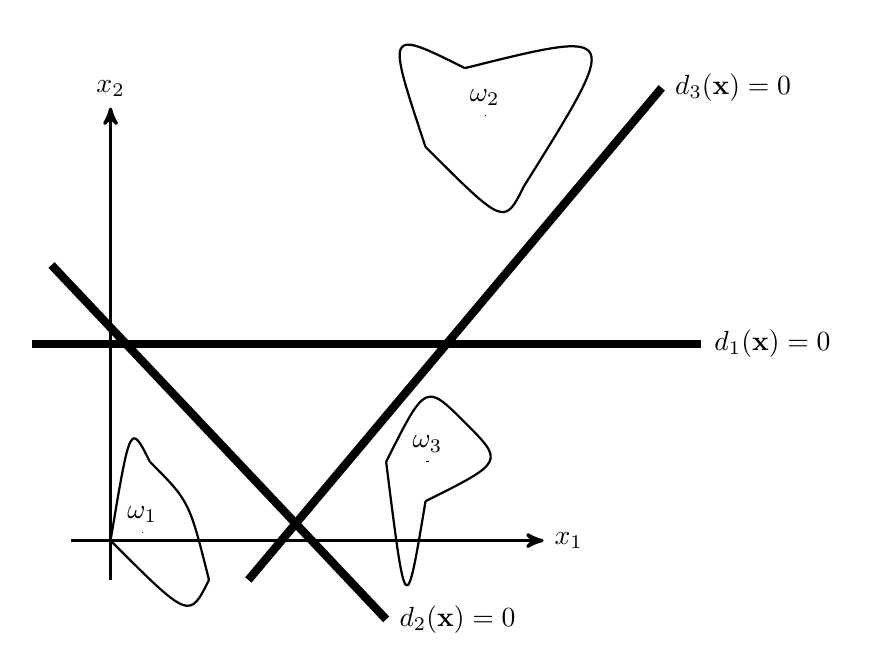
\begin{tikzpicture}[
    scale=5,
    axis/.style={very thick, ->, >=stealth'},
    important line/.style={thick},
    dashed line/.style={dashed, thin},
    pile/.style={thick, ->, >=stealth', shorten <=2pt, shorten
    >=2pt},
    every node/.style={color=black}
    ]
    
    %axis
    \draw[axis] (-0.1,0)  -- (1.1,0) node(xline)[right]
        {$x_1$};
    \draw[axis] (0,-0.1) -- (0,1.1) node(yline)[above] {$x_2$};
    
    %regions
    \draw[important line] (0,0) .. controls (0.2, -0.2) .. (0.25, -0.1);
    \draw[important line] (0.25,-0.1) .. controls (0.2, 0.1) .. (0.1, 0.2);
    \draw[important line] (0.1,0.2) .. controls (0.05, 0.3) .. (0, 0);
    
    \draw[important line] (.8,1) .. controls (1, 0.8) .. (1.05, 0.9);
    \draw[important line] (1.05,0.9) .. controls (1.3, 1.3) .. (.9, 1.2);
    \draw[important line] (.9,1.2) .. controls (0.7, 1.3) .. (.8, 1);
    
    \draw[important line] (.8,.1) .. controls (1, 0.2) .. (.9, 0.3);
    \draw[important line] (.9, 0.3) .. controls (.8, .4) .. (.7, .2);
    \draw[important line] (.7, .2) .. controls (.75, -.2) .. (.8,.1);
    
    %decision functions
    \draw[line width=3pt] (-.2, 0.5) -- (1.5, 0.5)  node[right, text width=5em]
    {$d_1(\mathbf{x}) = 0$};
    \draw[line width=3pt] (-.15, 0.7) -- (.7, -.2)  node[right, text width=5em]
    {$d_2(\mathbf{x}) = 0$};
    \draw[line width=3pt] (.35, -.1) -- (1.4, 1.15)  node[right, text width=5em]
    {$d_3(\mathbf{x}) = 0$};
    
    %regions names
    \draw (.08,0.02) -- (0.081,0.02) node[pos=.5,sloped,above] {$\omega_1$};
    \draw (.95,1.08) -- (.951,1.08) node[pos=.5,sloped,above] {$\omega_2$};
    \draw (.8,.2) -- (.81,.2) node[pos=.5,sloped,above] {$\omega_3$};
    
   \end{tikzpicture}
   \end{center}
   \end{figure}
  
  \item[\textbf{2. slučaj:}] Svaki razred uzoraka je separabilan sa svakim
  pojedinim razredom i to jednom decizijskom ravninom, tj. razredi su
  separabilni po parovima. Za razdvajanje nam je potrebno $\frac{M(M-1)}{2}$
  decizijskih ravnina. \\
  
  Strategija rješavanja ovog slučaja je upotribiti $\frac{c(c-1)}{2}$ linearnih
  funkcija odlučivanja tak oda sa svakom funkcijom odvojimo par razreda. Granica
  između razreda $\omega_i$ i $\omega_j$ je zadana s: $$d_{ij}(\mathbf{x}) =
  w_{ij1}x_1 + w_{ij2}x_2 + \ldots + w_{ijn}x_n + w_{ijn+1} = 0 $$
   \begin{figure}[H]
  \begin{center}
  
  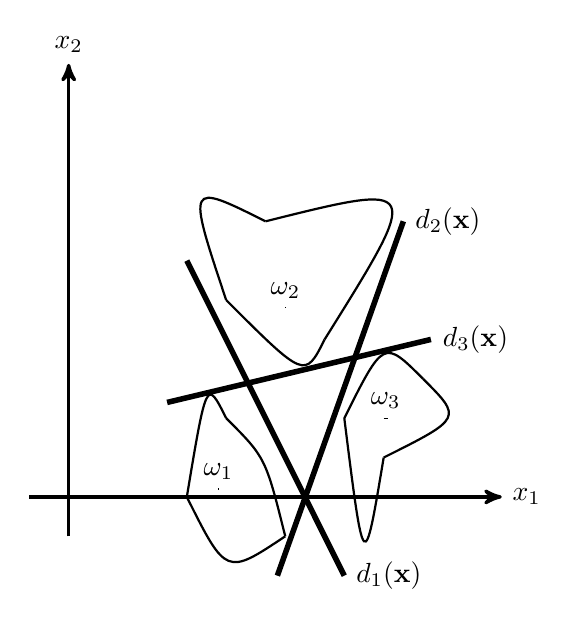
\begin{tikzpicture}[
    scale=5,
    axis/.style={very thick, ->, >=stealth'},
    important line/.style={thick},
    dashed line/.style={dashed, thin},
    pile/.style={thick, ->, >=stealth', shorten <=2pt, shorten
    >=2pt},
    every node/.style={color=black}
    ]
    
    %axis
    \draw[axis] (-0.1,0)  -- (1.1,0) node(xline)[right]
        {$x_1$};
    \draw[axis] (0,-0.1) -- (0,1.1) node(yline)[above] {$x_2$};
    
    %regions
    \draw[important line] (.3,0) .. controls (0.4, -0.2) .. (0.55, -0.1);
    \draw[important line] (0.55,-0.1) .. controls (0.5, 0.1) .. (0.4, 0.2);
    \draw[important line] (0.4,0.2) .. controls (0.35, 0.3) .. (.3, 0);
    
    \draw[important line] (.4,.5) .. controls (0.6, 0.3) .. (0.65, 0.4);
    \draw[important line] (.65,0.4) .. controls (.9, 0.8) .. (.5, .7);
    \draw[important line] (.5,.7) .. controls (0.3, .8) .. (.4, .5);
    
    \draw[important line] (.8,.1) .. controls (1, 0.2) .. (.9, 0.3);
    \draw[important line] (.9, 0.3) .. controls (.8, .4) .. (.7, .2);
    \draw[important line] (.7, .2) .. controls (.75, -.2) .. (.8,.1);
    
    %decision functions
    \draw[line width=2pt] (0.3, 0.6) -- (0.7, -0.2) node[right]
    {$d_1(\mathbf{x})$} ; 
    \draw[line width=2pt] (0.53, -0.2) -- (0.85, 0.7) node[right]
    {$d_2(\mathbf{x})$} ;
     \draw[line width=2pt] (0.25, .24) -- (0.92, 0.4) node[right]
     {$d_3(\mathbf{x})$} ;
    
    %regions names
    \draw (.38,0.02) -- (0.381,0.02) node[pos=.5,sloped,above] {$\omega_1$};
    \draw (.55,.48) -- (.551,.48) node[pos=.5,sloped,above] {$\omega_2$};
    \draw (.8,.2) -- (.81,.2) node[pos=.5,sloped,above] {$\omega_3$};
    
   \end{tikzpicture}
   \end{center}
   \end{figure}
  
  \item[\textbf{3. slučaj:}] Postoji $M$ decizijskih funkcija $d_k(\mathbf{x})
  = \mathbf{w}_k^T\mathbf{x}, \ k=1,2,\ldots,M$ sa svojstvom da $\mathbf{x}$
  pripada razredu $\omega_i$ ako vrijedi $$ d_i(\mathbf{x}) > d_j(\mathbf{x}) \
  \forall i\neq j. $$ To je poseban slučaj \textbf{2. slučaja} zato što možemo
  definirati slijedeće: $$d_{ij}(\mathbf{x}) = d_i(\mathbf{x}) - d_j(\mathbf{x})
  $$
  $$ \quad \quad = (\mathbf{w}_i - \mathbf{w}_j)^T\mathbf{x} $$
  $$  = \mathbf{w}_{ij}^T\mathbf{x} $$
  ako je $ d_i(\mathbf{x}) > d_j(\mathbf{x}) \ \forall i \neq i$, tada je
  $d_{ij}(\mathbf{x})>0 \ \forall j \neq i$, što znači da ako su srazredi
  separabilni za 3. slučaj, onda su automatski separabilni za 2.slučaj. \\
  
  Klasifikator za ovaj slučaj je ravnina:
  $$ (\mathbf{w}_i - \mathbf{w}_j)^T\mathbf{x} + (w_{in+1}-w_{jn+1}) = 0 .$$
  \marginpar[\textbf{Linearni klasifikator}]{\textbf{Linearni klasifikator}}
  Dobiveni klasifikator nazivamo \textbf{linearni klasifikator}.
\end{itemize}
  
\section{Određivanje funkcije odlučivanja}

Problem oblikovanja linearnog klasifikatora svodi se na određivanje
koeficijenata linearne funkcije odlučivanja:
$$ \mathbf{w} = \begin{bmatrix}
w_1 \\
w_2 \\
\vdots \\
w_n
\end{bmatrix}, $$
te koeficijenta $w_{n+1}$. \textit{Automatizaciju} postupka određivanja
koeficijenata linearne funkcije odlučivanja provest ćemo iterativnim postupkom
\marginpar[\textbf{Postupak učenja}]{\textbf{Postupak učenja}} \textbf{učenja}
koeficijenata linearne funkcije odlučivanja uporabom uzoraka iz skupa za učenje
(eng. \textit{training set}). \\

Skup za učenje sastoji se od $N$ uzoraka $\mathbf{x_1}, \mathbf{x_2},\ldots,
\mathbf{x_n}$ razvrstanih u dva razreda $\omega_1$ i $\omega_2$. Vektori uzoraka
$\mathbf{x_i}$ su \textbf{označeni} vektori (njihovu pripadnost razreda znamo)
pa ćemo njih \textbf{upotrijebiti za učenje} $d(\mathbf{x})$. \\

Kako bismo olakšali postupak učenja, povećat ćemo dimenzionalnost vektora
$\mathbf{w}$ za jedan:
$$ \mathbf{w} = \begin{bmatrix}
w_1 \\
w_2 \\
\vdots \\
w_n \\
1
\end{bmatrix} $$
radi elegantnijeg zapisa $d(\mathbf{x}) = \mathbf{w}^T\mathbf{x}$. Uspijemo li
odrediti takav vektor težinskih koeficijenata $\mathbf{x}$  tako da s pomoću
funkcije $f(\mathbf{x})$ pravilno razvrstamo sve uzorke iz skupa za učenje,
kažemo da su $\omega_1$ i $\omega_2$
\marginpar[\textbf{Linearno razdvojivi razredi}]{\textbf{Linearno razdvojivi
razredi}} \textbf{linearno razdvojivi}.

\begin{shaded}
Kažemo da je uzorak $\mathbf{x}$ pravilno razvrstan ako za sve $\mathbf{x}$ iz
$\omega_1$ vrijedi $\mathbf{w}^T\mathbf{x} > 0$ i ako za svaki $\mathbf{x}$ iz
$\omega_2$ vrijedi $\mathbf{w}^T\mathbf{x} < 0$. 
Gornje pravilo možemo zapisati kao jedinstven uvjet $\mathbf{w}^T\mathbf{x} > 0$
ako sve uzorke iz $\omega_2$ pomnožimo s -1.
\end{shaded}

To nas vodi na redefiniciju početnog problema: 
Tražimo vektor koeficijenata $\mathbf{w}$ linearne funkcije odlučivanja tako da
vrijedi $$\mathbf{w}^T\mathbf{x} > 0 $$ za svaki uzorak $\mathbf{x}$ iz skupa
uzoraka za učenje, odnosno:
$$ [\mathbf{x}]\mathbf{w} > 0 \quad \quad \forall \mathbf{x}   $$
$$ [\mathbf{x}] = \begin{bmatrix}
\mathbf{x}_1^T \\
\mathbf{x}_2^T \\
\vdots \\
\mathbf{x}_n^T
\end{bmatrix}  $$
pri čemu je $[\mathbf{x}]$ matrica svih uzoraka iz skupa za učenje, s tim da su
uzorci iz $\omega_2$ pomnoženi s -1. \\

\begin{shaded}
Primjer: \\

Zadani su slijedeći uzorci
\begin{figure}[H]
\begin{minipage}[b]{0.5\textwidth}
$$ \mathbf{x_1} = \begin{bmatrix}
0 \\
0
\end{bmatrix} $$
$$ \mathbf{x_3} = \begin{bmatrix}
1 \\
0
\end{bmatrix} $$
\end{minipage}
\begin{minipage}[b]{0.5\textwidth}
$$ \mathbf{x_2} = \begin{bmatrix}
0 \\
1
\end{bmatrix}$$

$$ \mathbf{x_4} = \begin{bmatrix}
1 \\
1
\end{bmatrix}, $$
\end{minipage}
\end{figure}

pri čemu je $\mathbf{x_1} \in \omega_1, \ \mathbf{x_2} \in \omega_1$, a
$\mathbf{x_3} \in \omega_2, \ \mathbf{x_4} \in \omega_2$. \\

Prvo što trebamo napraviti je povećati dimenzionalnost vektora:
\begin{figure}[H]
\begin{minipage}[b]{0.5\textwidth}
$$ \mathbf{x_1} = \begin{bmatrix}
0 \\
0 \\
1
\end{bmatrix} $$
$$ \mathbf{x_3} = \begin{bmatrix}
1 \\
0 \\ 
1
\end{bmatrix} $$
\end{minipage}
\begin{minipage}[b]{0.5\textwidth}
$$ \mathbf{x_2} = \begin{bmatrix}
0 \\
1 \\
1
\end{bmatrix}$$

$$ \mathbf{x_4} = \begin{bmatrix}
1 \\
1 \\
1
\end{bmatrix}, $$
\end{minipage}
\end{figure}

Zatim, pomnožimo sve elemente razreda $\omega_2$ s -1:
\begin{figure}[H]
\begin{minipage}[b]{0.5\textwidth}
$$ \mathbf{x_1} = \begin{bmatrix}
-1 \\
0 \\
-1
\end{bmatrix} $$

\end{minipage}
\begin{minipage}[b]{0.5\textwidth}
$$ \mathbf{x_2} = \begin{bmatrix}
-1 \\
-1 \\
-1
\end{bmatrix}$$
\end{minipage}
\end{figure}

Nakon toga, formirajmo matricu $[ \mathbf{x} ]$:
$$ [ \mathbf{x} ] = \begin{bmatrix}
0 & 0 & 1 \\
0 & 1 & 1 \\
-1 & 0 & -1 \\
-1 & -1 & -1
\end{bmatrix} $$

Nakon toga, potrebno je još samo riješiti slijedeći sustav nejednadžbi:
$$ [ \mathbf{x} ] \cdot \mathbf{w} > 0 $$
$$ \begin{bmatrix}
0 & 0 & 1 \\
0 & 1 & 1 \\
-1 & 0 & -1 \\
-1 & -1 & -1
\end{bmatrix} \cdot \begin{bmatrix}
w_1 \\
w_2 \\
w_3
\end{bmatrix} > \begin{bmatrix}
0 \\
0 \\
0 \\
0
\end{bmatrix} $$

\end{shaded}


\marginpar[\textbf{Razdvojni vektor}]{\textbf{Razdvojni vektor}} Vektor
$\mathbf{w}$ koji zadovoljava sustav linearnih nejednadžbi
$$[\mathbf{x}]\mathbf{w} > 0 $$ nazivamo \textbf{razdvojni vektor}.

 
\subsection{Gradijentni postupci određivanja razdvojnog vektora}

Problem pronalaska razdvojnog vektora često nije jednostavan te ga nije moguće
riješiti analitički. Da bismo našli hiperravninu koja razdvaja zadane klase,
moramo imati informaciju koliko je dobro naše trenutno rješenje te u kojem
smjeru se naše rješenje poboljšava. Definirajmo kriterijsku funkciju
\marginpar[\textbf{Kriterijska funkcija}]{\textbf{Kriterijska funkcija}} 
$J(\mathbf{a})$ koja je minimizirana  ako je $\mathbf{a}$ razdvojni vektor.
Smjer poboljšanja u tom nam slučaju govori \textbf{gradijent funkcije}. \\

Gradijent funkcije više varijabli, $f(\mathbf{y})$, gdje je $$ \mathbf{y} =
[x_1, x_2, \ldots, x_n]^T $$
definiran je kao 
$$ \mathbf{grad}f(\mathbf{y}) = \frac{df(\mathbf{y})}{d\mathbf{y}} =
\begin{bmatrix} \frac{\partial f}{\partial y_1} \\
\frac{\partial f}{\partial y_2} \\
\vdots \\
\frac{\partial f}{\partial y_n}
\end{bmatrix}. $$ 
Primjetimo da je gradijent skalarne funkcije vektorskog argumenta
\textbf{vektor}. Svaka komponenta promjene gradijenta predstavlja veličinu
promjene funkcije u smjeru komponente vektora te pri tome vrijedi: \\

\begin{itemize}
  \item  povećanje argumenata u smjeru pozitivnog gradijenta funkcije $f$ dovodi
  do \textbf{maksimuma} funkcije $f$
  \item povećanje argumenata u smjeru negativnog gradiejnta funkcije $f$ dovodi
  do \textbf{minimuma} funkcije $f$ \\
\end{itemize}


\begin{shaded}
\textit{Primjer:} \\

Uzmimo za primjer funkciju $J(w, 1) = (|w| - w)$. \\
Derivacije te funkcije je
$$ \frac{\partial J(w,1)}{\partial w} =
\mathbf{sgn}(w)-1 $$ gdje je 
$$ \mathbf{sgn}(x) = \left \{ \begin{array}{ll}
1, \quad \quad za \ x>0 \\
-1, \quad  za \ x<0
\end{array} \right.$$

\begin{figure}[H]

\begin{center}

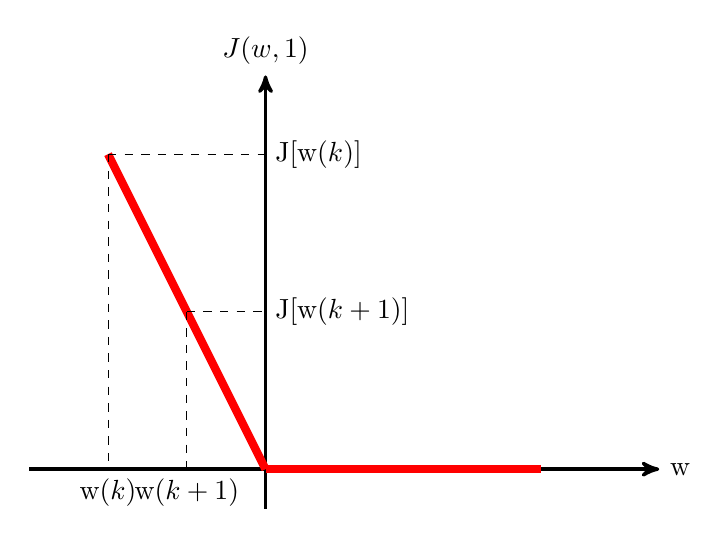
\begin{tikzpicture}[
    scale=5,
    axis/.style={very thick, ->, >=stealth'},
    important line/.style={thick},
    dashed line/.style={dashed, thin},
    pile/.style={thick, ->, >=stealth', shorten <=2pt, shorten
    >=2pt},
    every node/.style={color=black}
    ]
    
    % axis
    \draw[axis] (-0.6,0)  -- (1,0) node(xline)[right] {w};
    \draw[axis] (0,-0.1) -- (0,1) node(yline)[above] {$J(w,1)$};
    
    %function
    \draw[color=red, line width=3pt] (-0.4, 0.8) -- (0,0);
    \draw[color=red, line width=3pt] (0,0) -- (0.7,0);
    
    %marks
    \draw[dashed] (-0.4, 0.8) -- (0.0, 0.8) node[right] {J[w($k$)]};
    \draw[dashed] (-0.2, 0.4) -- (0.0, 0.4) node[right] {J[w($k+1$)]};
    \draw[dashed] (-0.4, 0.8) -- (-0.4, 0) node[below] {w($k$)};
    \draw[dashed] (-0.2, 0.4) -- (-0.2, 0) node[below] {w($k+1$)};
    
    
    
\end{tikzpicture} 

\end{center}
\end{figure}

Gradijent funkcije $J(w,1)$ jednaka je 
$$ \frac{\partial J(w,1)}{\partial w} = \left \{ \begin{array}{ll}
-2, \quad w\leq 0 \\
0, \quad \quad w>0
\end{array} \right. $$  

Ako promotrimo kretanje gradijenta funkcije $J(w,1)$, vidimo da se pri kretanju
$w(k) \mapsto w(k+1)$ povećavamo argument u smjeru negativne vrijednosti
gradijenta, tj. krećemo se prema minimumu funkcije.

\end{shaded}


Osnovna zamisao je odabrati takvu funkciju koja će dostići minimum kad je
ispunjen uvjet :
$$ \mathbf{w}^T\mathbf{x}_i > 0, \quad \quad \quad \forall i = 1,2,\ldots,N. $$

Pri tome zahtjevamo da izabrana funkcija ima samo jedan minimum te da je
funkcija $J(\mathbf{a})$ funkcija vektorskog argumenta $\mathbf{w}$. \\

\marginpar[\textbf{Gradijentni postupak}]{\textbf{Gradijentni postupak}}
Postupak pronalaženja minimuma funkcije pomoću gradijenta radimo tako da korak
po korak povećavamo argumenta $\mathbf{w}$ u smjeru negativnog argumenta
funkcije $J(\mathbf{w}, \mathbf{x})$ sve dok nije postignut minimum kriterijske
funkcije $J(\mathbf{w}, \mathbf{x})$. \\

Ako je $\mathbf{w}(k)$ vrijednost $\mathbf{w}$ u $k$-tom koraku, tada vrijednost
u koraku $(k+1)$ definiramo kao 
$$ \mathbf{w}(k+1) = \mathbf{w}(k) - c \cdot \left \{ \frac{\partial
J(\mathbf{w}(k), \mathbf{x})}{\partial \mathbf{w}(k)} \right \}, $$
gdje je $c$ pozitivna konstanta različita od 0 koja određuje veličinu
korekcije.\\

Korekcija se više ne izvodi kada je $\frac{\partial
J(\mathbf{w}(k), \mathbf{x})}{\partial \mathbf{w}(k)} = 0$, što je i uvjet za
minimum. \\

\begin{shaded}
\textbf{Podsjetnik o deriviranju funkcije} \\




\begin{figure}[H]



\centering

\begin{tabular}{c|c}
\textbf{Funkcija} & \textbf{Derivacija} \\
\hline \\
$c$ (konst.) & 0 \\
$x^n$ & $nx^{n-1}$ \\
$\frac{1}{x}$ & $-\frac{1}{x^2}$ \\
$\frac{1}{x^n}$ & $-\frac{n}{x^{n+1}}$ \\
$\sqrt{x}$ & $\frac{1}{2\sqrt{x}}$ \\
$\sqrt[n]{x}$  & $\frac{1}{n\sqrt[n]{x^{n-1}}}$ \\
$e^x$ & $e^x$ \\
$a^x$ & $a^x\mathbf{ln}a$ \\
$\mathbf{ln}x$ & $\frac{1}{x}$ \\
\end{tabular}
 


\end{figure}


\textbf{Deriviranje linearnih funkcija}

\begin{center}
$$ \frac{d}{d\mathbf{x}}(\mathbf{x}^T\mathbf{A})= \mathbf{A} $$
$$ \frac{d}{d\mathbf{x}}(\mathbf{x}^T) = \mathbf{I} $$
$$ \frac{d}{d\mathbf{x}}(\mathbf{x}^T\mathbf{a})=
\frac{d}{d\mathbf{x}}(\mathbf{a}^T\mathbf{x}) = \mathbf{a}$$
$$ \frac{d}{d\mathbf{X}}(\mathbf{a}^T\mathbf{X}\mathbf{b}) =
\mathbf{a}\mathbf{b}^T $$
$$ \frac{d}{d\mathbf{X}}(\mathbf{a}^T\mathbf{X}\mathbf{a}) =
\frac{d}{d\mathbf{X}}(\mathbf{a}^T\mathbf{X}^T\mathbf{a}) =
\mathbf{a}\mathbf{a}^T $$
$$ \frac{d}{d\mathbf{x}}(\mathbf{x}^T\mathbf{C}\mathbf{x}) = (\mathbf{C} +
\mathbf{C}^T)\mathbf{x} $$
\flushright{ ako je $\mathbf{C}=\mathbf{C}^T$ onda je
$\frac{d}{d\mathbf{x}}(\mathbf{x}^T\mathbf{C}\mathbf{x}) =
2\mathbf{C}\mathbf{x}$}
$$ \frac{d}{d\mathbf{x}}(\mathbf{x}^T\mathbf{x}) = 2\mathbf{x}$$
$$ \frac{d}{d\mathbf{x}}(\mathbf{A}\mathbf{x} +
\mathbf{b})(\mathbf{D}\mathbf{x} + \mathbf{e}) =
\mathbf{A}^T(\mathbf{D}\mathbf{x} + \mathbf{e}) + \mathbf{D}^T(\mathbf{A}\mathbf{x} +
\mathbf{b}) $$
\end{center}


\textbf{Nekoliko pravila}






\end{shaded}

  
 
\subsection{Perceptron}
\subsection{Ho-nešto algoritam}

\chapter{Fisherova linearna diskriminanta}

\marginpar[\textbf{Fisherova analiza}]{\textbf{Fisherova analoza}}Fisherova
linearna diskriminanta je još  jedan pristup linearnoj klasifikaciji koji se
temelji na ideji da se početni  $d$-dimenzionalan vektor značajki $\mathbf{x}$
reducira na jednu dimenziju ($\Re^n \mapsto \Re^1 $) te ga  tada upotrijebiti za
klasifikaciju. \\

\begin{figure}[H]
\begin{center}
\includegraphics[scale=0.5]{./pics/fisher_beg}
\end{center}
\end{figure}

Cilj Fisherove linearne diskriminante je pronaći orijentaciju pravca na koji se
projiciraju $d-$dimenzionalni uzorci $\mathbf{x}_i, i = 1,2,\ldots,n$ ali tako
da su projicirani uzorci separabilni. Upravo to je cilja \textit{klasične}
diskriminantne analize. \\

Za skup od $n$ $d$-dimenzionalnih uzoraka, od kojih $n_1$ uzoraka čine podskup
$\mathcal{D}_1$ i $n_2$ uzoraka koji čine podskup $\mathcal{D}_2$, tvorimo
linearnu kombinaciju komponenti $\mathbf{x}$: 
$$ y_i = \mathbf{w}^T\mathbf{x}_i, \quad i=1,2,\ldots,n $$
Tako dobivamo odgovarajući skup od $n$ uzoraka $y_1,y_2,\ldots,y_n$ koji su
podjeljeni u podskupove $\mathcal{Y}_1$ i $\mathcal{Y}_2$. Ako je pri tome
$\lVert  \mathbf{w} \rVert = 1$, svaki $y_i$ je projekcija odgovarajućeg vektora
$\mathbf{x}_i$ na pravac u smjeru $\mathbf{w}$.

\begin{figure}[H]
\begin{center}
\includegraphics[scale=0.5]{./pics/fisher_projekcija}
\end{center}
\end{figure}

Veličina vektora $\mathbf{w}$ nema posebno značenje, ona samo skalira $y_i$.
Važan je smjer od $\mathbf{w}$! \\

Ako zamislimo da uzorci iz $\omega_1$ čine nakupinu, te da uzorci iz $\omega_2$
čine drugu nakupinu, \textbf{želimo da projekcije na pravac određen s
$\mathbf{w}$ budu takva da su dobro razdvojive}.

\begin{figure}[H]
\begin{center}
\includegraphics[scale=0.5]{./pics/fisher_primjer}
\end{center}
\end{figure}

Uzmimo za mjeru odvojivosti između projiciranih točaka razliku srednjih
vrijednosti projiciranih uzoraka. Neka je
$$ \mathbf{m}_i = \frac{1}{n_i}\sum\limits_{\mathbf{x} \in
\mathcal{D}_i}\mathbf{x}; \quad i=1,2$$
Srednja vrijednosti projiciranih uzoraka: 
$$ \widetilde{m}_i = \frac{1}{n_i}\sum\limits_{y \in
\mathcal{Y}_i}y $$
Da li je udaljenost srednjoh vrijednosti projiciranih uzoraka \textit{dobra
mjera}?

\begin{figure}[H]
\begin{center}
\includegraphics[scale=.5]{./pics/fisher_dobramjeraupitnik}
\end{center}
\end{figure} 

Neka je $\widetilde{m}_i$ projekcija vektora $\mathbf{m}_i$:
$$ \widetilde{m}_i = \frac{1}{n_i}\sum\limits_{\mathbf{x} \in
\mathcal{D}_i}\mathbf{w}^T\mathbf{x} = \mathbf{w}\mathbf{m}_i $$
tada je razlika između srednjih vrijednosti projiciranih uzoraka:
$$ | \widetilde{m}_1 - \widetilde{m}_2 | = | \mathbf{w}(\mathbf{m}_1 -
\mathbf{m}_2) | $$

Primjetimo da razliku možemo učiniti proizvoljno velikom skaliranjem
$\mathbf{w}$. da bismo dobili dobro odvajanje projiciranih podataka želimo da
\textbf{udaljenost} između srednjih vrijednosti projiciranih točaka bude
relativno velika u odnosu na \textbf{neku mjeru standardne devijacije za svaki
razred.} \\

Sada kriterijsku funkciju možemo definirati kao
$$ J(\mathbf{w}) = \frac{(razlika \ srednjih \ vrijednosti)^2}{varijanca \
uzoraka \ unutar \ razred} = \frac{ (\widetilde{m}_1 - \widetilde{m}_2 )^2
}{\sigma_{\mathcal{Y}_1}^2 + \sigma_{\mathcal{Y}_2}^2}. $$

Fisherova linearna diskriminanta određuje da linearna funkcija
$$\mathbf{w}^T\mathbf{x} $$ za koju je kriterijska funkcija $J(\mathbf{w})$
\textbf{maksimalna} vodi najboljem razdvajanju između projiciranih skupova. \\

Umjesto varijanci $\sigma_i$  možemo definirati raspršenost projiciranih
podataka unutar razreda $C_i$ kao:
$$ \widetilde{\mathbf{s}}^2_i = \sum\limits_{y \in \mathcal{Y}_i}(y -
\widetilde{\mathbf{m}}_i)^2. $$
Tada je $\frac{1}{n}( \widetilde{\mathbf{s}}^2_1 + \widetilde{\mathbf{s}}^2_2)$
procjena varijance podataka a $\widetilde{\mathbf{s}}^2_1 +
\widetilde{\mathbf{s}}^2_2$ je ukupna mjera raspršenosti projiciranih podataka
unutar razreda (eng. \textit{total within-class scatter}). \\

Kako želimo $J(\cdot)$ dobiti kao funkciju od vektora $\mathbf{w}$, definirajmo
matricu:
$$ \mathcal{S}_i = \sum\limits_{\mathbf{x} \in \mathcal{D}_i}(\mathbf{x} -
\mathbf{m}_i)(\mathbf{x} - \mathbf{m}_i)^T $$
kao raspršenost unutar razreda $\omega_i$. 
Dalje: 
$$ \mathcal{S}_W = \mathcal{S}_1 + \mathcal{S}_2 $$
$$  \widetilde{\mathbf{s}}^2_i = \sum\limits_{\mathbf{x} \in
\mathcal{D}_i}(\mathbf{w}^T\mathbf{x} - \mathbf{w}^T\mathbf{m}_i)^2 $$
$$ = \sum\limits_{\mathbf{x} \in
\mathcal{D}_i}\mathbf{w}^T\underbrace{(\mathbf{x} -  \mathbf{m}_i)(\mathbf{x} -
\mathbf{m}_i)}_{\mathcal{S}_i}^T\mathbf{w} $$
 
$$  \widetilde{\mathbf{s}}^2_i = \mathbf{w}^T\mathcal{S}_i\mathbf{w}. $$ \\

Suma $\widetilde{\mathbf{s}}^2_1 + \widetilde{\mathbf{s}}^2_2$ tada je jednaka 
$$ \mathbf{w}^T \mathcal{S}_w \mathbf{w} .$$ 
Matrica $\mathcal{S}_w$ simetrična je i pozitivno semidefinitna te je obično
nesingularna ako je $n>d$. \\

Slično gornjemu, možemo definirati i slijedću vrijednost:
$$ (\widetilde{\mathbf{m}}_1 - \widetilde{\mathbf{m}}_2)^2 =
(\mathbf{w}^T\widetilde{\mathbf{m}}_1 - \mathbf{w}^T\widetilde{\mathbf{m}}_2)^2
$$
$$ = \mathbf{w}^T(\widetilde{\mathbf{m}}_1 -
\widetilde{\mathbf{m}}_2)(\widetilde{\mathbf{m}}_1 -
\widetilde{\mathbf{m}}_2)^T\mathbf{w} $$ 
$$ = \mathbf{w}^T\mathcal{S}_B\mathbf{w}.$$

Matricu $\mathcal{S}_B$ predstavlja raspršenost projiciranih uzoraka između
klasa (eng. \textit{between-class scatter matrix}).
Za matricu $\mathcal{S}_B$ vrijedi sve što vrijedi i za matricu $\mathcal{S}_W$.
Sada kriterijsku funkciju možemo definirati kao: 
$$ J(\mathbf{w}) =
\frac{\mathbf{w}^T\mathcal{S}_B\mathbf{w}}{\mathbf{w}^T\mathcal{S}_W\mathbf{w}}.
$$
Za određivanje matrica $\mathcal{S}_B$ i $\mathcal{S}_W$ koristimo uzorke iz
skupova $\mathcal{D}_1$ i $\mathcal{D}_2$. \\

Odredimo maksimum $J(\mathbf{w})$:
$$ \frac{\partial J(\mathbf{w})}{\partial \mathbf{w}} = 0 $$
$$ = \frac{\partial J(\mathbf{w})}{\partial \mathbf{w}} =
\frac{\partial}{\partial \mathbf{w}} \left (
\frac{\mathbf{w}^T\mathcal{S}_B\mathbf{w}}{\mathbf{w}^T\mathcal{S}_W\mathbf{w}}
\right ) = 0 $$
$$ \frac{(\mathbf{w}^T\mathcal{S}_W\mathbf{w})\frac{\partial}{\partial
\mathbf{w}}(\mathbf{w}^T\mathcal{S}_B\mathbf{w}) -
(\mathbf{w}^T\mathcal{S}_B\mathbf{w})\frac{\partial}{\partial
\mathbf{w}}(\mathbf{w}^T\mathcal{S}_W\mathbf{w})
}{(\mathbf{w}^T\mathcal{S}_W\mathbf{w})^2} = 0 $$
$$ (\mathbf{w}^T\mathcal{S}_W\mathbf{w})\cdot 2\mathcal{S}_B\mathbf{w} -
(\mathbf{w}^T\mathcal{S}_B\mathbf{w})\cdot 2\mathcal{S}_W\mathbf{w} = 0  $$
$$\mathcal{S}_w\mathbf{w}(\mathbf{w}^T\mathcal{S}_B\mathbf{w})
(\mathbf{w}^T\mathcal{S}_W\mathbf{w})^{-1} = \mathcal{S}_B\mathbf{w} $$
Ako to zapišemo u obliku:
$$ \lambda \mathcal{S}_W\mathbf{w} = \mathcal{S}_B\mathbf{w} $$

gdje je $\lambda$ skalar iznosa $(\mathbf{w}^T\mathcal{S}_B\mathbf{w})
(\mathbf{w}^T\mathcal{S}_W\mathbf{w})^{-1}$, vidimo da se naš problem svodi na
\textbf{generalizirani problem svojstvenog vektora}. \\

Ako $\mathcal{S}_W^{-1}$ postoji onda je \textbf{smjer} $\mathbf{w}$ jednak 
$$ \hat{\mathbf{w}} = (\mathcal{S}_W^{-1}\mathcal{S}_B)\mathbf{w}.$$
Za naš slučaj nije potrebno to rješavati na način da tražimo svojstvene
vrijednosti i svojstvene vektore za $\mathcal{S}_W^{-1}\mathcal{S}_B)\mathbf{w}$
zato što je $\mathcal{S}_B\mathbf{w}$ \textbf{uvijek usmjeren kao}
$\mathbf{m}_1-\mathbf{m}_2 $! \\
Budući da nas zanima samo smjer vektora $\mathbf{w}$, a ne faktor skaliranja,
možemo napisati rješenje za $\mathbf{w}$:
$$ \mathbf{m}_1 = \begin{bmatrix}
m_{11} \\
m_{12} \\
m_{13}
\end{bmatrix} \quad \mathbf{m}_2 = \begin{bmatrix}
m_{21} \\
m_{22} \\
m_{23}
\end{bmatrix} $$
$$ \mathcal{S}_B = ( \mathbf{m}_1 - \mathbf{m}_2 ) \cdot (\mathbf{m}_1 -
\mathbf{m}_2)^T. $$

Pokažimo da je $\mathcal{S}_b\mathbf{w}$ zaista usmjeren u smjeru $\mathbf{m}_1
- \mathbf{m}_2$ :
$$ \mathcal{S}_B\mathbf{w} = ( \mathbf{m}_1 - \mathbf{m}_2 ) 
\cdot \underbrace{(\mathbf{m}_1
- \mathbf{m}_2)^T \mathbf{w}}_{k}  $$

$$ \mathcal{S}_B\mathbf{w} = ( \mathbf{m}_1 - \mathbf{m}_2 ) \cdot \mathbf{w} $$
Iz toga vidimo da je $\mathcal{S}_B\mathbf{w}$ usmjeren u smjeru $\mathbf{m}_1 -
\mathbf{m}_2$. \\

Iz toga slijedi da 
$$ \hat{\mathbf{w}} = \mathcal{S}_W(\mathbf{m}_1 - \mathbf{m}_2) ,$$
te da  $\mathbf{w}$ u skladu s Fisherovom linearnog diskriminantom određuje
linearnu funkciju koja maksimizira omjer između raspršenja između razreda  i
raspršenja unutar razreda.




\end{document}
